% !TEX root = ../../../main.tex
% 来源：中学数学实验教材·第二册（几何）
% 章节：轨迹与作图 / 轨迹
% 原始文件：5.tex，行 143-153
% 类型：tikz
% ---
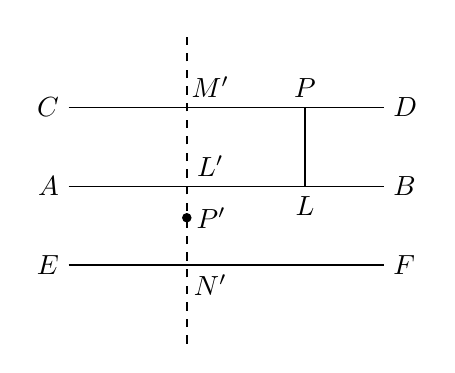
\begin{tikzpicture}
\draw (0,0)node[left]{$E$}--(4,0)node[right]{$F$};
\draw (0,1)node[left]{$A$}--(4,1)node[right]{$B$};
\draw (0,2)node[left]{$C$}--(4,2)node[right]{$D$};
\draw[dashed, thick] (1.5,-1)--(1.5,3);
\draw[thick] (3,1)node[below]{$L$}--(3,2)node[above]{$P$};
\node at (1.8,0)[below]{$N'$};
\node at (1.8,1)[above]{$L'$};
\node at (1.8,2)[above]{$M'$};
\draw (1.5,.6) [fill=black] circle (1.5pt) node[right]{$P'$};
\end{tikzpicture}
